% Drawing 85/05-2 -- folder 85, batch 05, archive page 95 (PDF page 96).
% Transcription: figures. En haut à gauche, un treillis au crayon et à l'encre, en forme de losanges, dont les flèches montent de gauche à droite ; au-dessous et au milieu, un grand treillis encadré d'une courbe fermée, dont les sommets sont $\mathfrak{A}_2 = 1$, $\mathbb{Z}_2$, $\mathfrak{S}_2$, $\mathfrak{S}'_2$, $\mathfrak{S}''_2$, $\mathfrak{S}_{22}$, $\mathfrak{S}^{*}_{22}$, $\mathfrak{A}_3$, $\mathbb{D}_3$, $\mathfrak{S}_3$, $\mathfrak{S}'_3$, $\mathbb{D}'_3$, $\mathbb{Z}_6$, $\mathbb{Z}'_6$, $\widetilde{\mathfrak{S}}_3$, $\widetilde{\mathfrak{S}}'_3$, $\mathfrak{A}_5$, $\mathfrak{S}_5$, avec à gauche un petit losange $\mathbb{D}_4$, $\mathbb{Z}_4$, $\mathbb{D}_2$, $\mathbb{E}_2$ et en dessous $\mathfrak{A}_4$, $\mathfrak{S}_4$, $\mathbb{D}_2$, $\mathbb{D}_4$ ; certaines flèches sont en pointillé. Au milieu, un octaèdre au crayon. À droite, un diagramme d'ensembles : les points $1, 2, 3, 4, 5$ dans des ovales marqués $\mathfrak{S}_2$ (autour de $1, 2$), $\mathfrak{S}'_2$ (autour de $4, 5$), $\mathfrak{S}_3$ et $\mathfrak{S}'_3$
% Kind: sheet of subgroup lattices of S5, pencil octahedron, set diagram. Method 2 (schematic redraw from the facsimile). Status: partial.
% Notes: Whole upper half of the sheet. Top left: the lattice of diamonds, its arrows rising left to right (nodes placed, labels left out, as in the transcription which names none). Middle: the pencil octahedron, schematised. Below: the large lattice inside a closed curve, its vertices labelled after the transcription (positions read on the facsimile; the reading of some vertices, e.g. E2 and S*22, is uncertain), plain and dashed arrows placed between node centres; the small diamond D4, Z4, D2, E2 on the left drawn faint; A4, S4 below it are not drawn (they belong to the lower lattice). Right: the set diagram, points 1..5 in ovals S2, S2', S3, S3'. Left out: the text, the boxed isomorphisms, the circled marginal note and its outline, the count table; the lower perspective lattice (described in a \note of the transcription, not by this mark).
% Coordinates: 1 unit = 1 mm = 1/100 of the crop width (bbox in page fractions: [0.05, 0.12, 0.95, 0.58]).
% Redrawn by Claude (claude-opus-5-5), issue #73, 2026-11-07; not checked by a human; not compiled (no TeX in the session).
% Rights: reproduces part of the work -- behind RENDER_TRANSCRIPTS, never published by itself.
\documentclass[tikz,border=3pt]{standalone}
\usepackage{amsmath,amssymb}
\usetikzlibrary{patterns,arrows.meta}
\tikzset{pencil/.style={black!45}, struck/.style={black!35}, mark/.style={circle,draw,inner sep=1.3pt}, pt/.style={circle,fill,inner sep=0.9pt}, opt/.style={circle,draw,fill=white,inner sep=1.1pt}}
\begin{document}
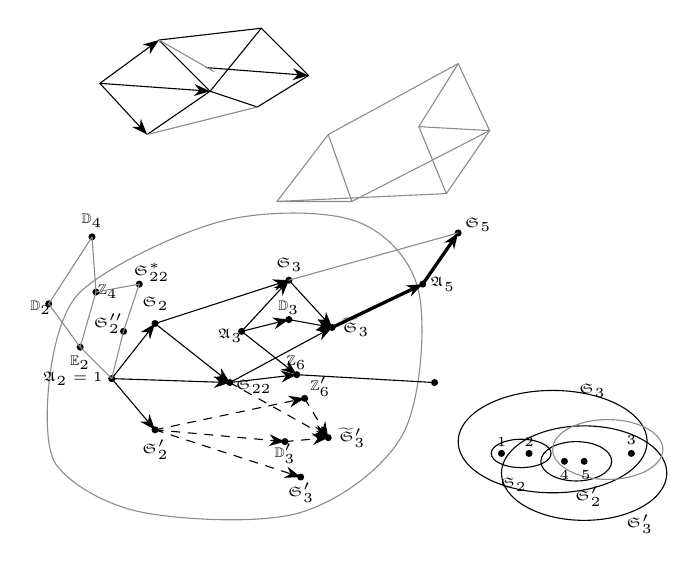
\begin{tikzpicture}[x=1mm,y=1mm,line cap=round,line join=round,font=\scriptsize]
\draw[-{Stealth[length=2mm]}] (14.5,-13.5) -- (22,-8);
\draw[-{Stealth[length=2mm]}] (14.5,-13.5) -- (20.5,-20);
\draw[-{Stealth[length=2mm]}] (14.5,-13.5) -- (28.5,-14.5);
\draw (22,-8) -- (28.5,-14.5);
\draw (20.5,-20) -- (28.5,-14.5);
\draw (22,-8) -- (35,-6.5);
\draw (28.5,-14.5) -- (35,-6.5);
\draw (35,-6.5) -- (41,-12.5);
\draw (28.5,-14.5) -- (34.5,-16.5);
\draw (34.5,-16.5) -- (41,-12.5);
\draw[-{Stealth[length=2mm]}] (28,-11.5) -- (41,-12.5);
\draw[pencil] (22,-8) -- (29,-12);
\draw[pencil] (20.5,-20) -- (34.5,-16.5);
\draw[pencil] (37,-28.5) -- (43.5,-20) -- (46.5,-28.5) -- cycle;
\draw[pencil] (55,-19) -- (60,-11) -- (64,-19.5) -- (58.5,-27.5) -- cycle;
\draw[pencil] (43.5,-20) -- (60,-11);
\draw[pencil] (37,-28.5) -- (58.5,-27.5);
\draw[pencil] (46.5,-28.5) -- (64,-19.5);
\draw[pencil] (55,-19) -- (64,-19.5);
\draw[pencil] plot[smooth, tension=0.55] coordinates {(8,-52) (12,-40) (30,-31) (47,-31) (55,-40) (53,-58) (40,-68) (20,-68) (9,-62) (8,-52)};
\node[pt] at (16,-51) {};
\node[pt] at (21.5,-44) {};
\node[pt] at (21.5,-57.5) {};
\node[pt] at (31,-51.5) {};
\node[pt] at (19.5,-39) {};
\node[pt] at (17.5,-45) {};
\node[pt] at (12,-47) {};
\node[pt] at (13.5,-33) {};
\node[pt] at (14,-40) {};
\node[pt] at (8,-41.5) {};
\node[pt] at (32.5,-45) {};
\node[pt] at (38.5,-43.5) {};
\node[pt] at (38.5,-38.5) {};
\node[pt] at (44,-44.5) {};
\node[pt] at (39.5,-50.5) {};
\node[pt] at (40.5,-53.5) {};
\node[pt] at (38,-59) {};
\node[pt] at (43.5,-58.5) {};
\node[pt] at (40,-63.5) {};
\node[pt] at (55.5,-39) {};
\node[pt] at (60,-32.5) {};
\node[inner sep=1pt] at (11,-51) {\tiny $\mathfrak{A}_2 = 1$};
\node[inner sep=1pt] at (21.5,-41.5) {\tiny $\mathfrak{S}_2$};
\node[inner sep=1pt] at (21.5,-60) {\tiny $\mathfrak{S}'_2$};
\node[inner sep=1pt] at (34,-52) {\tiny $\mathfrak{S}_{22}$};
\node[inner sep=1pt] at (21,-37.5) {\tiny $\mathfrak{S}^{*}_{22}$};
\node[inner sep=1pt] at (15.5,-44) {\tiny $\mathfrak{S}''_2$};
\node[inner sep=1pt] at (12,-49) {\tiny $\mathbb{E}_2$};
\node[inner sep=1pt] at (13.5,-31) {\tiny $\mathbb{D}_4$};
\node[inner sep=1pt] at (15.5,-40) {\tiny $\mathbb{Z}_4$};
\node[inner sep=1pt] at (7,-42) {\tiny $\mathbb{D}_2$};
\node[inner sep=1pt] at (31,-45.5) {\tiny $\mathfrak{A}_3$};
\node[inner sep=1pt] at (38.5,-42) {\tiny $\mathbb{D}_3$};
\node[inner sep=1pt] at (38.5,-36.5) {\tiny $\mathfrak{S}_3$};
\node[inner sep=1pt] at (47,-44.5) {\tiny $\widetilde{\mathfrak{S}}_3$};
\node[inner sep=1pt] at (39.5,-49) {\tiny $\mathbb{Z}_6$};
\node[inner sep=1pt] at (42.5,-52) {\tiny $\mathbb{Z}'_6$};
\node[inner sep=1pt] at (38,-60.5) {\tiny $\mathbb{D}'_3$};
\node[inner sep=1pt] at (46.5,-58.5) {\tiny $\widetilde{\mathfrak{S}}'_3$};
\node[inner sep=1pt] at (40,-65.5) {\tiny $\mathfrak{S}'_3$};
\node[inner sep=1pt] at (58,-39) {\tiny $\mathfrak{A}_5$};
\node[inner sep=1pt] at (62.5,-31.5) {\tiny $\mathfrak{S}_5$};
\draw[-{Stealth[length=2mm]}] (16,-51) -- (21.5,-44);
\draw[-{Stealth[length=2mm]}] (16,-51) -- (31,-51.5);
\draw[-{Stealth[length=2mm]}] (16,-51) -- (21.5,-57.5);
\draw[-{Stealth[length=2mm]}] (21.5,-44) -- (31,-51.5);
\draw[-{Stealth[length=2mm]}] (21.5,-44) -- (38.5,-38.5);
\draw[-{Stealth[length=2mm]}] (31,-51.5) -- (44,-44.5);
\draw[-{Stealth[length=2mm]}] (32.5,-45) -- (38.5,-38.5);
\draw[-{Stealth[length=2mm]}] (32.5,-45) -- (38.5,-43.5);
\draw[-{Stealth[length=2mm]}] (38.5,-43.5) -- (44,-44.5);
\draw[-{Stealth[length=2mm]}] (38.5,-38.5) -- (44,-44.5);
\draw[-{Stealth[length=2mm]}] (32.5,-45) -- (39.5,-50.5);
\draw[pencil] (38.5,-38.5) -- (60,-32.5);
\draw[very thick,-{Stealth[length=2mm]}] (44,-44.5) -- (55.5,-39);
\draw[very thick,-{Stealth[length=2mm]}] (55.5,-39) -- (60,-32.5);
\draw[pencil] (16,-51) -- (17.5,-45);
\draw[pencil] (17.5,-45) -- (19.5,-39);
\draw[-{Stealth[length=2mm]}] (31,-51.5) -- (39.5,-50.5);
\draw[dashed,-{Stealth[length=2mm]}] (21.5,-57.5) -- (40.5,-53.5);
\draw[dashed,-{Stealth[length=2mm]}] (21.5,-57.5) -- (38,-59);
\draw[dashed,-{Stealth[length=2mm]}] (31,-51.5) -- (43.5,-58.5);
\draw[dashed,-{Stealth[length=2mm]}] (40.5,-53.5) -- (43.5,-58.5);
\draw[dashed,-{Stealth[length=2mm]}] (38,-59) -- (43.5,-58.5);
\draw[dashed,-{Stealth[length=2mm]}] (21.5,-57.5) -- (40,-63.5);
\draw[pencil] (13.5,-33) -- (14,-40);
\draw[pencil] (14,-40) -- (12,-47);
\draw[pencil] (8,-41.5) -- (13.5,-33);
\draw[pencil] (8,-41.5) -- (12,-47);
\draw[pencil] (12,-47) -- (16,-51);
\draw[pencil] (14,-40) -- (19.5,-39);
\draw (39.5,-50.5) -- (57,-51.5);
\node[pt] at (57,-51.5) {};
\draw (72,-59) ellipse[x radius=12, y radius=6.5];
\draw (76,-63) ellipse[x radius=10.5, y radius=6];
\draw (68,-60.5) ellipse[x radius=3.8, y radius=1.8];
\draw (75,-61.5) ellipse[x radius=4.5, y radius=2.5];
\draw[pencil] (79,-60) ellipse[x radius=7, y radius=3.8];
\node[pt] at (65.5,-60.5) {};
\node[pt] at (69,-60.5) {};
\node[pt] at (73.5,-61.5) {};
\node[pt] at (76,-61.5) {};
\node[pt] at (82,-60.5) {};
\node[inner sep=1pt] at (65.5,-59) {\tiny $1$};
\node[inner sep=1pt] at (69,-59) {\tiny $2$};
\node[inner sep=1pt] at (73.5,-63.2) {\tiny $4$};
\node[inner sep=1pt] at (76.2,-63.2) {\tiny $5$};
\node[inner sep=1pt] at (82,-58.8) {\tiny $3$};
\node[inner sep=1pt] at (67,-64.5) {\tiny $\mathfrak{S}_2$};
\node[inner sep=1pt] at (76.5,-66) {\tiny $\mathfrak{S}'_2$};
\node[inner sep=1pt] at (77,-52.5) {\tiny $\mathfrak{S}_3$};
\node[inner sep=1pt] at (83,-69.5) {\tiny $\mathfrak{S}'_3$};
\end{tikzpicture}
\end{document}
